\documentclass[12pt,utf8]{scrartcl}
\usepackage[ngerman]{babel}
\usepackage{hyperref}
\hypersetup{
	colorlinks=true,	
	linkcolor=blue,     
	citecolor=blue,     
	filecolor=blue,     
	urlcolor=blue     	
}
\usepackage{etoolbox}
\apptocmd{\UrlBreaks}{\do\-\do\%\do\.}{}{}
\usepackage[ngerman]{varioref}
\usepackage{amsmath,amssymb,latexsym,amsfonts,amsthm,amsbsy,qtree}
\usepackage{url}
\usepackage[printonlyused]{acronym}
\usepackage[utf8]{inputenc} 
\usepackage{graphicx}
\usepackage{float}
\usepackage{fancyhdr}
\usepackage{booktabs}
\usepackage{enumitem}
\usepackage[justification=centering]{caption}
\usepackage[numbers]{natbib}
\bibliographystyle{plainnat}
\usepackage{pdfpages}

\newcommand{\teilnehmerI}{Tom Dombeck}
\newcommand{\mattI}{4510671} 
\newcommand{\mailI}{todo@uni-bremen.de}
\newcommand{\teilnehmerII}{Andreas Schwarz}
\newcommand{\mattII}{4250572}
\newcommand{\mailII}{andreas4@uni-bremen.de}
\newcommand{\teilnehmerIII}{Lasse Warnke}
\newcommand{\mattIII}{4515161}
\newcommand{\mailIII}{lwarnke@uni-bremen.de}
\newcommand{\thisgroup}{A01}
\newcommand{\abgabedatum}{23.12.2018}
\newcommand{\nummer}{2}
\newcommand{\thema}{Integrierte Anwendungssysteme, Big Data}
\newcommand{\thistutor}{Tim Haß}
\newcommand{\thissemester}{WiSe 2018/19}
\newcommand{\thiscourse}{Wirtschaftsinformatik 1}
\newcommand{\thisshortcourse}{WI1}

\pagestyle{fancy}
\fancyhead{} 												
\fancyhead[LO,RE]{\thissemester \\ \thisshortcourse} 
\fancyhead[RO,LE]{TutorIn: \thistutor \\ Gruppe: \thisgroup }
\fancyfoot{} 											
\cfoot{\thepage} 										
\setlength{\headsep}{2cm} 								

\begin{document}
\begin{titlepage}
	\vspace*{\baselineskip}		
	\centering					
	\LARGE							
	\thiscourse \\ 					
	\vspace{1cm}					
	{\Huge 							
	\textbf{Abgabe \nummer: \thema}} \\ 
	\vspace{1.5cm} 					
	TutorIn: \thistutor \\ 		
	\abgabedatum \\ 				
	\vfill 							
	Gruppe: \thisgroup \\ 			
	\vspace{.5cm} 					
	\large 							
	\begin{tabular}{c|c|c} 		
	\teilnehmerI	& \teilnehmerII & \teilnehmerIII \\ 
	\mattI	& \mattII &  \mattIII\\ 
	\mailI	& \mailII & \mailIII \\ 
	\end{tabular} 
\end{titlepage}

\thispagestyle{empty}
\tableofcontents
\newpage
\setcounter{page}{1}

\section*{Aufgabe 2.1}
\addcontentsline{toc}{section}{Aufgabe 2.1}
\subsection*{\label{sub:thema}1. Probleme der dezentralen Lösung}
\addcontentsline{toc}{subsection}{1. Probleme der dezentralen Lösung}

Um die Probleme welche das dezentrale System dem Bremer Polizeipräsidium verursacht zu verstehen muss man erstmal seinen Aufbau kennen. Aktuell besitz jede Abteilung, oder zumindest jede genannte, ihr eigenens IT-System. Das bedeuted entweder ein stark personalisiertes oder sogar selbst entwickeltes System. 

Diese Insellösungen sorgen für eine ganze Menge Probleme. Vor allem wenn man das jetzige System mit einem zentralisierten IT-System vergleicht. 
Das erste und offensichtlichste Problem ist die kompatibilität der einzelnen Systeme. Also der Datenaustasch zwischen den einzelene Abteilungen des Polizeipräsidiums. Durch die wahrscheinlich stark unterschiedlichen Systeme ist es nicht unbedingt gewährleistet das diese miteinander kompatibel sind und dadurch effizient Daten zwischen den einzelnen Abteilungen ausgetauscht werden können (wenn dies überhaupt ohne Umweg möglich ist).

Dies führt gleichzeitig natürlich auch zu einem erhöhten Administrationsaufwand um die unterschiedlichen Systeme am laufen zu halten. Da viele verschiedenen IT-Systeme gibt wird eine größere Anzahl an Administratoren gebraucht welche sich auch noch  mit vielen verschiedenen Systemen auskennen müssen. Dies führt wahrscheinlisch zu höheren Personalkosten als auch zu mehr Ausfällen als wenn es ein zentrales IT-System geben würde.

Ein weiterer nicht zu vernachlässigender Punkt ist die Sicherheit welche durch die große Anzahl an verschiedenen System natürlich ebenfalls beeinträchtigt ist. Im vergleich zu einem zentralen System ist es bei den vielen verschiedenen Abteilungssystemen schwieriger einen einheitlichen Sicherheitsstandard einzuhalten.

Ein Problem welches schon bei der Administration angesprochen wurde ist die Ausfallsicherheit eines solchen dezentralen Systems. Durch die verschiedenen Syteme und dadurch auch verteilte Aufmerksamkeit der Administratoren auf dei verschiedenen Syteme ist es natürlich schwieriger eine große Anzahl von Systemen 24/7 am laufen zu halten als ein Sytem welches die ungeteilte Aufmerksamgeit aller Administratoren genießt.


\subsection*{\label{sub:thema}2. Sytemlandkarte mit Sollkonzept}
\addcontentsline{toc}{subsection}{2. Sytemlandkarte mit Sollkonzept}

Grundlegend werden bei deisem Konzept alle Abteilungen mit allen verbunden. Es entsteht ein zentrales Serversystem und eine zentrale Datenbank oder zumindest zetral zugängliche Datenbanken für die normal anfallenden Daten. Für besonders vertrauliche Daten wie z.B. Einstzpläne oder die Liste der aktuell sich in Polizeigewahrsam befindenden Personen wird eine externe Datenbank angelegt auf welche nur von den jeweiligen Abteilungen zugegriffen werden kann.

Durch die zentrale Infrastruktur um die zentrale Datenbank herum können Schnittstellen zwischen den einzelnen Abteilungen relativ einfach realisiert werden. Dies ist auch wichtig, da es zwischen so gut wie allen Abteilungen auch Schnittstellen benötigt werden. 


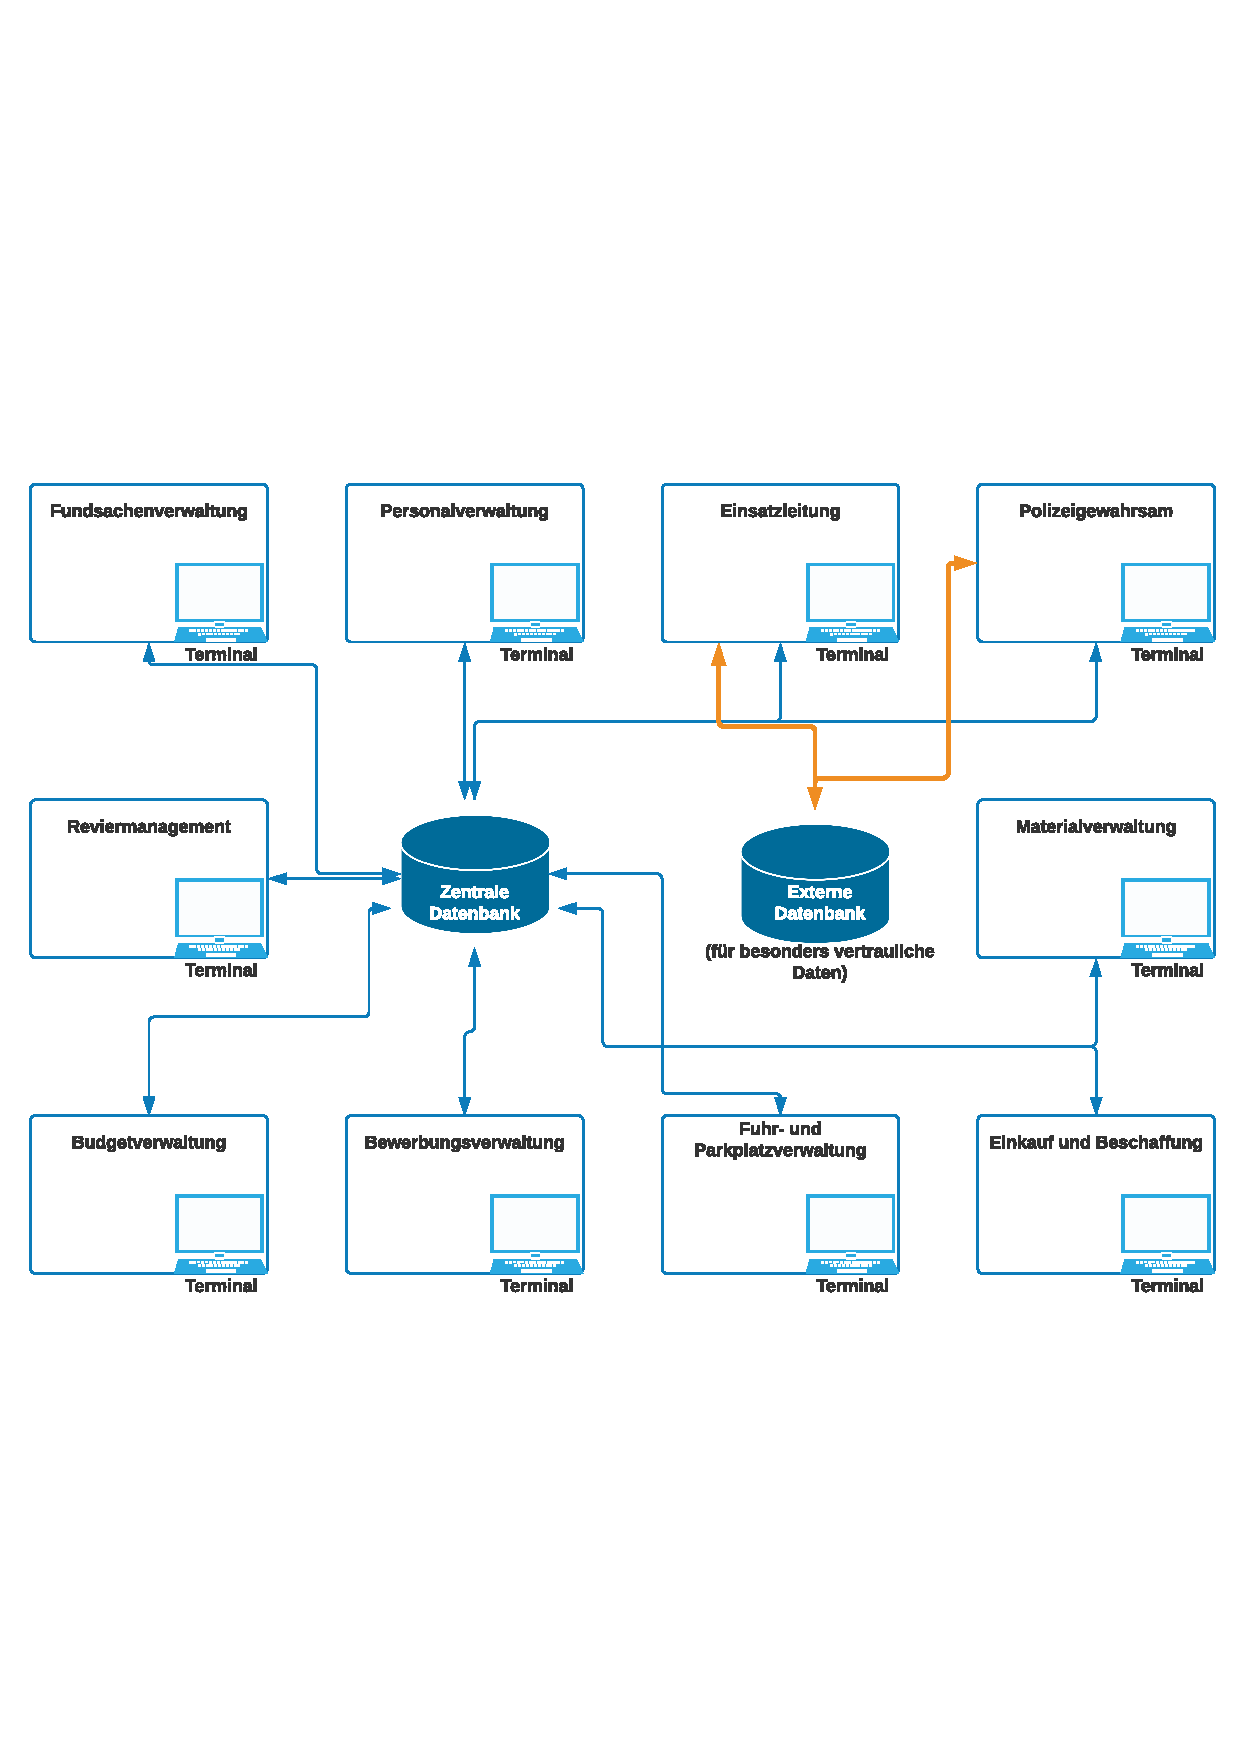
\includepdf[pages=1]{NetworkDiagram.pdf}



\subsection*{\label{Aufgabe 2.1.3}3. ERP-Module für die Polizei Bremen}
\addcontentsline{toc}{subsection}{3. ERP-Module für die Polizei Bremen}

ERP-Systeme sind modular aufgebaut und somit an einzelne Kunden besser individuell anpassbar. Moderne ERP-Systeme umfassen oft eine große Zahl an Funktionsbereichen oder Modulen. 

- Fundsachenverwaltung -> 
- Personalverwaltung -> Personalwirtschaft
- Einsatzleitung -> 
- Materialverwaltung -> 
- Polizeigewahrsam -> 
- Reviermanagement -> 
- Budgetverwaltung -> Finanz- und Rechnungswesen
- Bewerbungsverwaltung -> 
- Fuhr- und Parkplatzverwaltung -> 
- Einkauf und Beschaffung -> 

\newpage
\subsection*{4. Einführung eines ERP-Systems für die Polizei Bremen}
\addcontentsline{toc}{subsection}{4. Einführung eines ERP-Systems für die Polizei Bremen}

Wir würden Herrn Techniksturm wie folgt überzeugen:

ERP-Systeme verursachen eine höhere Produktivität. Sie bieten dem Unternehmen eine einheitliche Organisation, da alle Daten in einem System vorhanden und auch abrufbar sind, wodurch die Leitung extrem vereinfacht wird. Generell wird die Koordination in einem Unternehmen durch das gemeinsame Nutzen von Daten sehr stark verbessert, schneller und auch einfacher. So können Kosten und Produktionszeit für ein Unternehmen gesenkt und seine Effektivität erhöht werden\cite{Nwankpa2015}.

Es gibt verschiedene Herangehensweisen um ein ERP-System neu in ein Unternehmen einzuführen. Man kann entweder schrittweise vorgehen (step-by-step), indem man für eine bestimmte Zeit einen Parallelbetrieb hat, man macht einen sogenannten "Big Bang", bei dem man das komplette System an einem Stichtag einführt, oder man führt zunächst in einem kleinen Unternehmensbereich entweder step-by-step oder als "Big Bang" einen Prototypen ein, sodass die dort gewonnene Erfahrung später nützlich sein kann und gegebenenfalls anfallende Probleme dort schon entdeckt und gelöst werden können. Natürlich haben alle Varianten ihre Vor- und Nachteile. So müssen bei einer schrittweisen Einführung die alten Systeme und das neue ERP-System temporäre Schnittstellen haben, damit alle Systeme weiterhin funktionieren. Dies ist bei einem "Big Bang" natürlich nicht nötig, da alle alten Systeme auf einen Schlag ersetzt werden. Auf der anderen Seite muss die Umstellung auf ein anderes System natürlich vorbereitet werden. Alle Mitarbeiter müssen z.B. geschult und mit dem neuen System vertraut gemacht werden. Dies ist natürlich einfacher, wenn man ein System nur nach und nach z.B. an verschiedenen geographischen Standorten oder nach Modulen geordnet einführt, da man so eine kleinere Anzahl an Leuten zur gleichen Zeit schulen muss\cite{Jacob2008}. 

Für die Polizei Bremen würden wir ein schrittweise eingeführtes ERP-System empfehlen, weil es sich mit rund 2.500 Angestellten um ein recht großes "Unternehmen" handelt, das zudem geographisch weit über das Land Bremen verstreut ist\cite{PolizeiBremen}. Hinzu kommt, dass eine step-by-step Einführung ein relativ kleines Risiko im Vergleich zum "Big Bang" bietet. Außerdem ist eine Aktualisierung des Systems nicht dringend notwendig sondern nur wünschens- und empfehlenswert, sodass die Zeit, die das Projekt in Anspruch nimmt, eine untergeordnete Rolle spielt\cite{Hansmann2005}. 

Bei der Einführung eines ERP-Systems handelt es sich um ein Projekt, weil es sich um ein einmaliges Ereignis handelt und nur das Ergebnis vorher fest definiert ist. Zunächst muss man sich für eines der auf dem Markt verfügbaren ERP-Systeme entscheiden. Am meisten in Deutschland verbreitet sind ERP-Systeme von SAP, gefolgt von Systemen von Oracle\citep{Foerster2008}. Dies ist der Schritt der Systemauswahl. Da alle Geschäftsprozesse, die unterstützt werden sollen, und somit auch alle ERP-Module, die für die Polizei Bremen in Frage kommen, schon geklärt sind (siehe Aufgabe 2.1.2 und 2.1.3), ist ein weiterer Schritt auf dem Weg zur Einführung eines ERP-Systems, die Vorstudie und die Istanalyse, schon gemacht. Es folgt ein Sollkonzept, dass die Erwartungen an das System und dessen Möglichkeiten vorab definiert. Danach kommt die Realisierung. Das System wird customized und getestet. Zudem wird in diesem Schritt angefangen erste Endanwender zu schulen und auf das neue System vorzubereiten. Hierauf folgt die wirkliche Einführung des Systems. Es wird vor Ort installiert und gegebenenfalls noch optimiert. Alle benötigten und für das System erforderlichen Daten werden an das neue System übergeben. Der finale Schritt ist die Inbetriebnahme. Das Projekt wird bewertet und es wird ein Abschlussbericht verfasst. Natürlich muss auch in Zukunft weiter an dem System gearbeitet, es stetig weiterentwickelt und optimiert werden. Außerdem müssen alle Angestellten mit dem System vertraut gemacht werden\cite{Hansmann2005}.

Wichtig bei einem solchen Projekt ist die vollständige Dokumentation des Projektes. Mit Hilfe der Dokumentation und den Erwartungen, die man an das neue System und an das Projekt hat, sollte man nach jedem Phasenabschluss überprüfen, ob man seine Erwartungen erfüllt oder man hinterher hängt. Sollte dies der Fall sein, muss dies sofort der Projektleitung mitgeteilt werden, sodass diese Maßnahmen treffen kann, um wieder den Erwartungen gerecht zu werden\cite{Foerster2008}. Hierzu zählen auch Anpassungen der einzelnen Module des Systems, sodass sie besser auf das Unternehmen zutreffen. 

An dem Projekt Einführung eines ERP-Systems müssen zunächst alle betroffenen Funktionsbereiche beteiligt werden, da sie am besten darüber Aufschluss geben können, was benötigt wird. Sie sind die Fachexperten. Außerdem sollten ebenfalls alle Hierarchieebenen des Unternehmens vertreten sein, da sie alle unterschiedliche Wünsche und Forderungen an das System stellen. Auch sollten alle geographischen Standorte sich mit einbringen können. Zum Schluss fehlen noch Experten für das Prozessmanagement, die den Fach- und Softwareexperten bei der Umsetzung ihrer Ideen helfen können, und für die Software, die sich um den IT-Teil des Projektes kümmern\cite{Hansmann2005}.

\newpage
\section*{Aufgabe 2.2}
\addcontentsline{toc}{section}{Aufgabe 2.2}

\newpage
\begin{flushleft}
\addcontentsline{toc}{section}{Literaturverzeichniss}
\bibliography{Literaturdatenbank}
\end{flushleft}
\end{document}
